\subsection*{全体概要：この章で学ぶこと}
\addcontentsline{toc}{subsection}{全体概要：この章で学ぶこと}

この章は、ソフトウェア開発の最初だけでなく、設計・実装・テスト・保守まで影響する「要求」を扱う。ここでいう要求とは、利用者や顧客の希望だけでなく、業務規則、法令、標準、運用上の制約、性能や安全性の水準、予算や納期の制約まで含み得る。

\SmallHead{到達目標}
この章を読み終えると、次のことができるようになる。
\begin{itemize}
\item 「要求」「機能要求」「非機能要求」「技術制約」「サービス品質制約」を区別できる。
\item 要求をどこから集めるか、どのように引き出すかを説明できる。
\item 要求が曖昧・不完全・矛盾している場合に、何を確認すべきかを説明できる。
\item 要求を文章・受け入れ基準・モデルとして記録する方法の違いを説明できる。
\item 要求の妥当性確認、変更管理、優先順位付け、追跡可能性の役割を説明できる。
\end{itemize}

\SmallHead{学習順序}
初学者は、まず「要求とは何か」と「要求の分類」を押さえる。その後、「要求をどう集めるか」「どう分析するか」「どう書くか」「どう確認するか」「どう変化に対応するか」という流れで読むとよい。

\begin{figure}[htbp]
\centering
\IfFileExists{assets/generated_figures/ch01/fig-ch01-01.png}{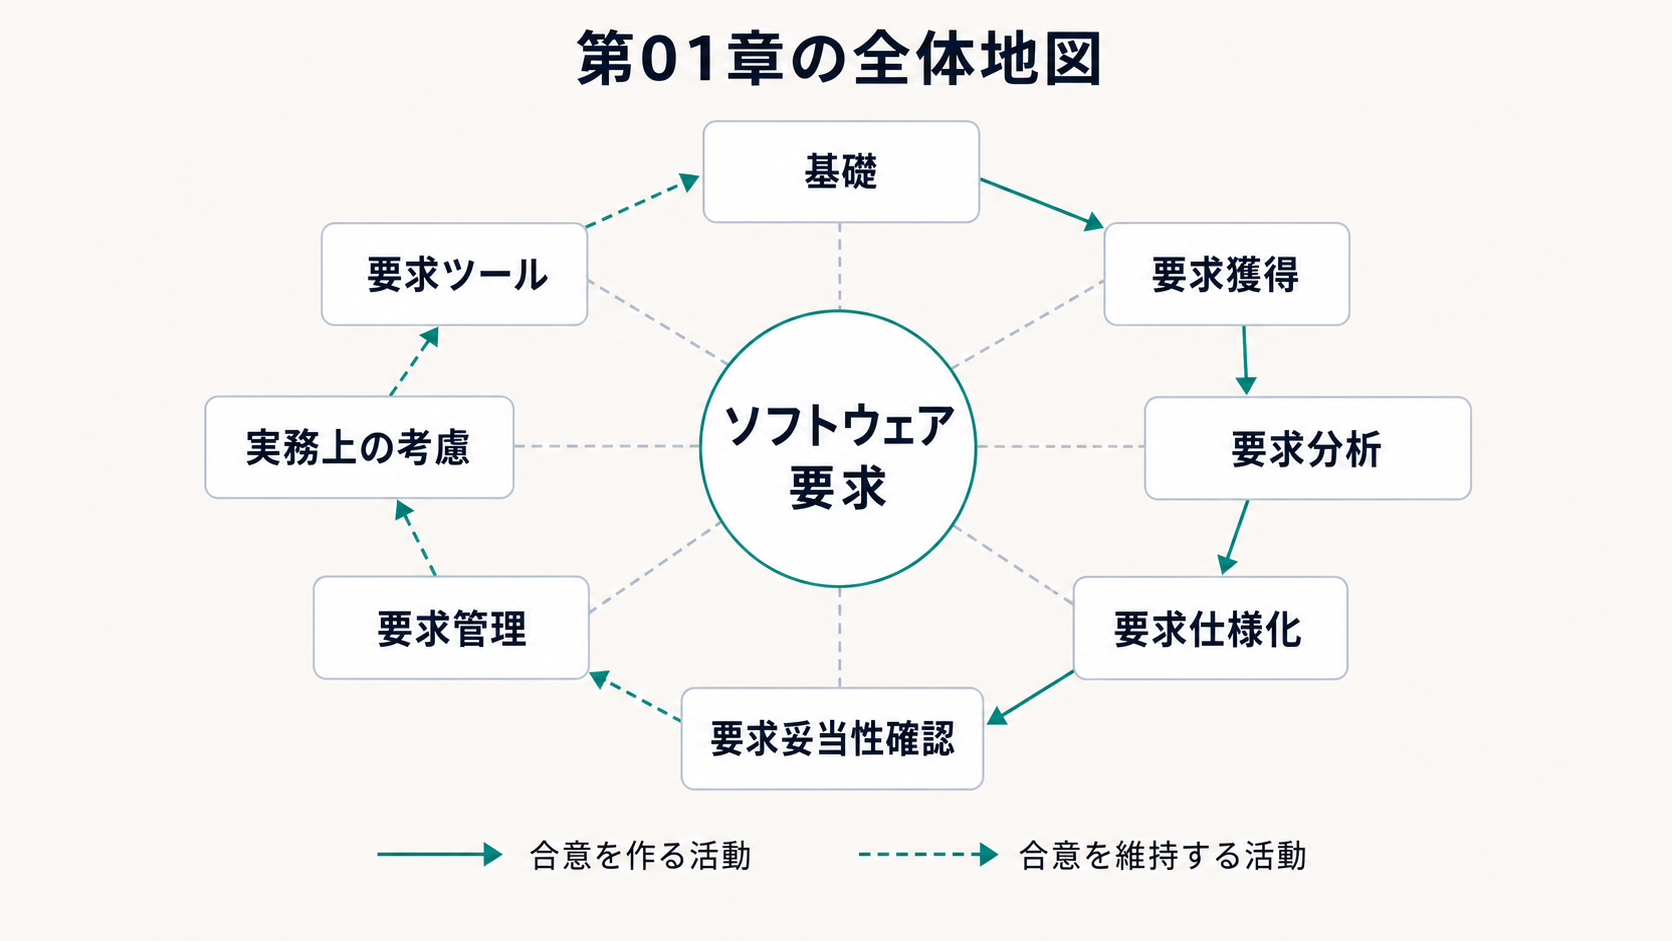
\includegraphics[width=0.96\linewidth]{assets/generated_figures/ch01/fig-ch01-01.png}}{\fbox{\parbox[c][48mm][c]{0.9\linewidth}{\centering 画像生成待ち\\第01章の全体地図}}}
\caption{第01章の全体地図}
\label{fig:ch01-01}
\end{figure}

\subsubsection*{最初に必要な用語}
\addcontentsline{toc}{subsubsection}{最初に必要な用語}

\par\smallskip\noindent\refstepcounter{table}\label{tab:ch01-01}\textbf{表 \thetable: 第01章 ソフトウェア要求 表01}\par\smallskip
\begin{tabularx}{0.97\linewidth}{@{}p{.25\linewidth}X@{}}
\toprule
用語 & 初学者向けの説明 \\
\midrule
\term{ソフトウェア} & プログラムだけでなく、データ、設定、操作手順、関連文書を含むことがある。 \\
\term{要求} & 何かを達成するために満たすべき条件・能力・制約。 \\
\term{利害関係者} & 開発結果に影響を与える、または影響を受ける人・組織。顧客、利用者、運用担当、規制当局など。 \\
\term{システム} & ソフトウェア、ハードウェア、人、手順、設備などが組み合わさって目的を達成するもの。 \\
\term{仕様} & 要求や設計などを、関係者が共有できるように記録したもの。 \\
\term{妥当性確認} & 「これを作れば本当に相手の問題を解決できるか」を確認すること。 \\
\term{追跡可能性} & 要求が設計、コード、テスト、利用者文書などとどうつながるかをたどれること。 \\
\bottomrule
\end{tabularx}
